%% 5 Lorenzo
%5. My profile. Where the registered user can:
%    a. Update profile information (ie: picture, description, email address);
%    b. Have an overview of all the orders he made on the website;
\subsection{UC15 - Modifica informazioni profilo}
\label{UC15}
\begin{figure}[H]
    \centering
    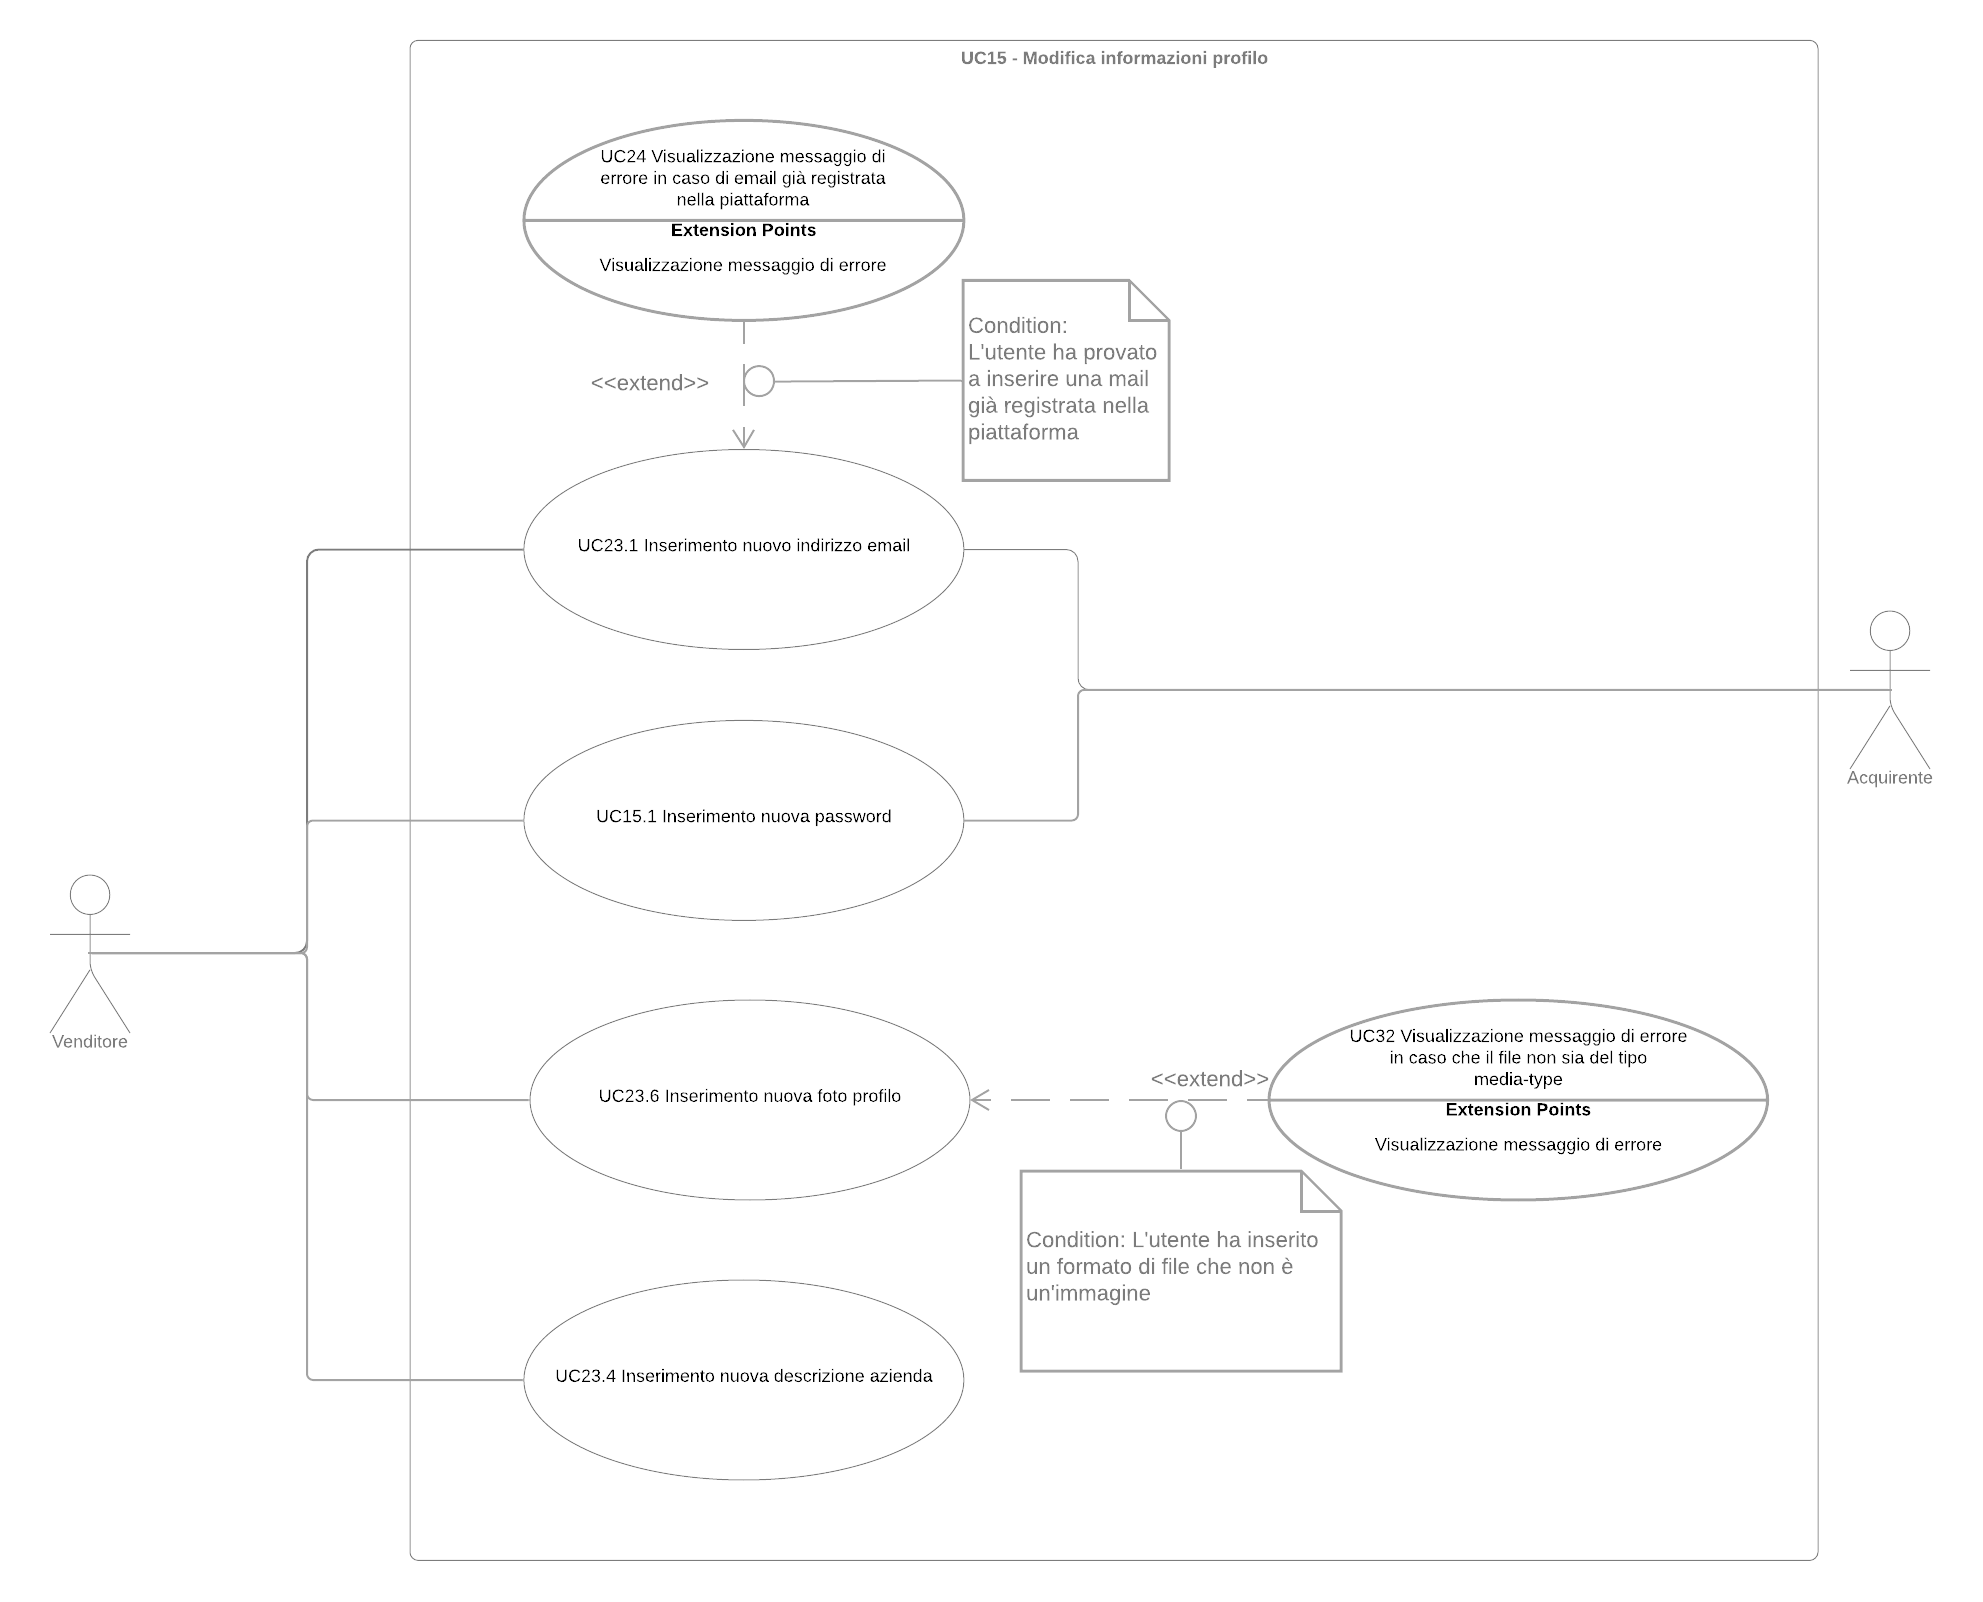
\includegraphics[width=\textwidth]{Immagini/DiagrammiUC/UC15ModificaInformazioniProfilo}
    \caption{Diagramma di UC15: Modifica informazioni profilo} 
    \label{fig:VisualizzazioneProdottiNelCarrello}
\end{figure}

L'acquirente o il venditore vuole modificare le sue informazioni personali.
\begin{itemize}
    \item \textbf{Attori primari:} Acquirente; Venditore.
    \item \textbf{Precondizione:} L'attore si trova nella pagina personale (UC3.2.1) e ha premuto sul link per la modifica delle informazioni.
    \item \textbf{Postcondizione:} L'attore ha aggiornato le sue informazioni personali.
    \item \textbf{Scenario Principale:} L'attore ha premuto sul link per la modifica delle informazioni personali e può così iniziare a modificarle. I campi che si possono modificare sono:
    \begin{itemize}
        \item per l'acquirente:
        \begin{itemize}
            \item (UC23.1) - Inserimento nuovo indirizzo e-mail.
            \item (UC15.1) - Inserimento nuova password.
        \end{itemize}
        \item per il venditore:
        \begin{itemize}
            \item (UC23.1) - Inserimento nuovo indirizzo e-mail.
            \item (UC15.1) - Inserimento nuova password.
            \item (UC23.6) - Inserimento nuova foto profilo.
            \item (UC23.4) - Inserimento nuova descrizione azienda.
        \end{itemize}
    \end{itemize}
    \item \textbf{Estensioni:}
    \begin{itemize}
        \item (UC24) - Visualizzazione messaggio di errore in caso di email già registrata nella piattaforma.
    \end{itemize}
\end{itemize}

\subsubsection{UC15.1 - Inserimento nuova password}
\label{UC15.1}

\begin{figure}[H]
    \centering
    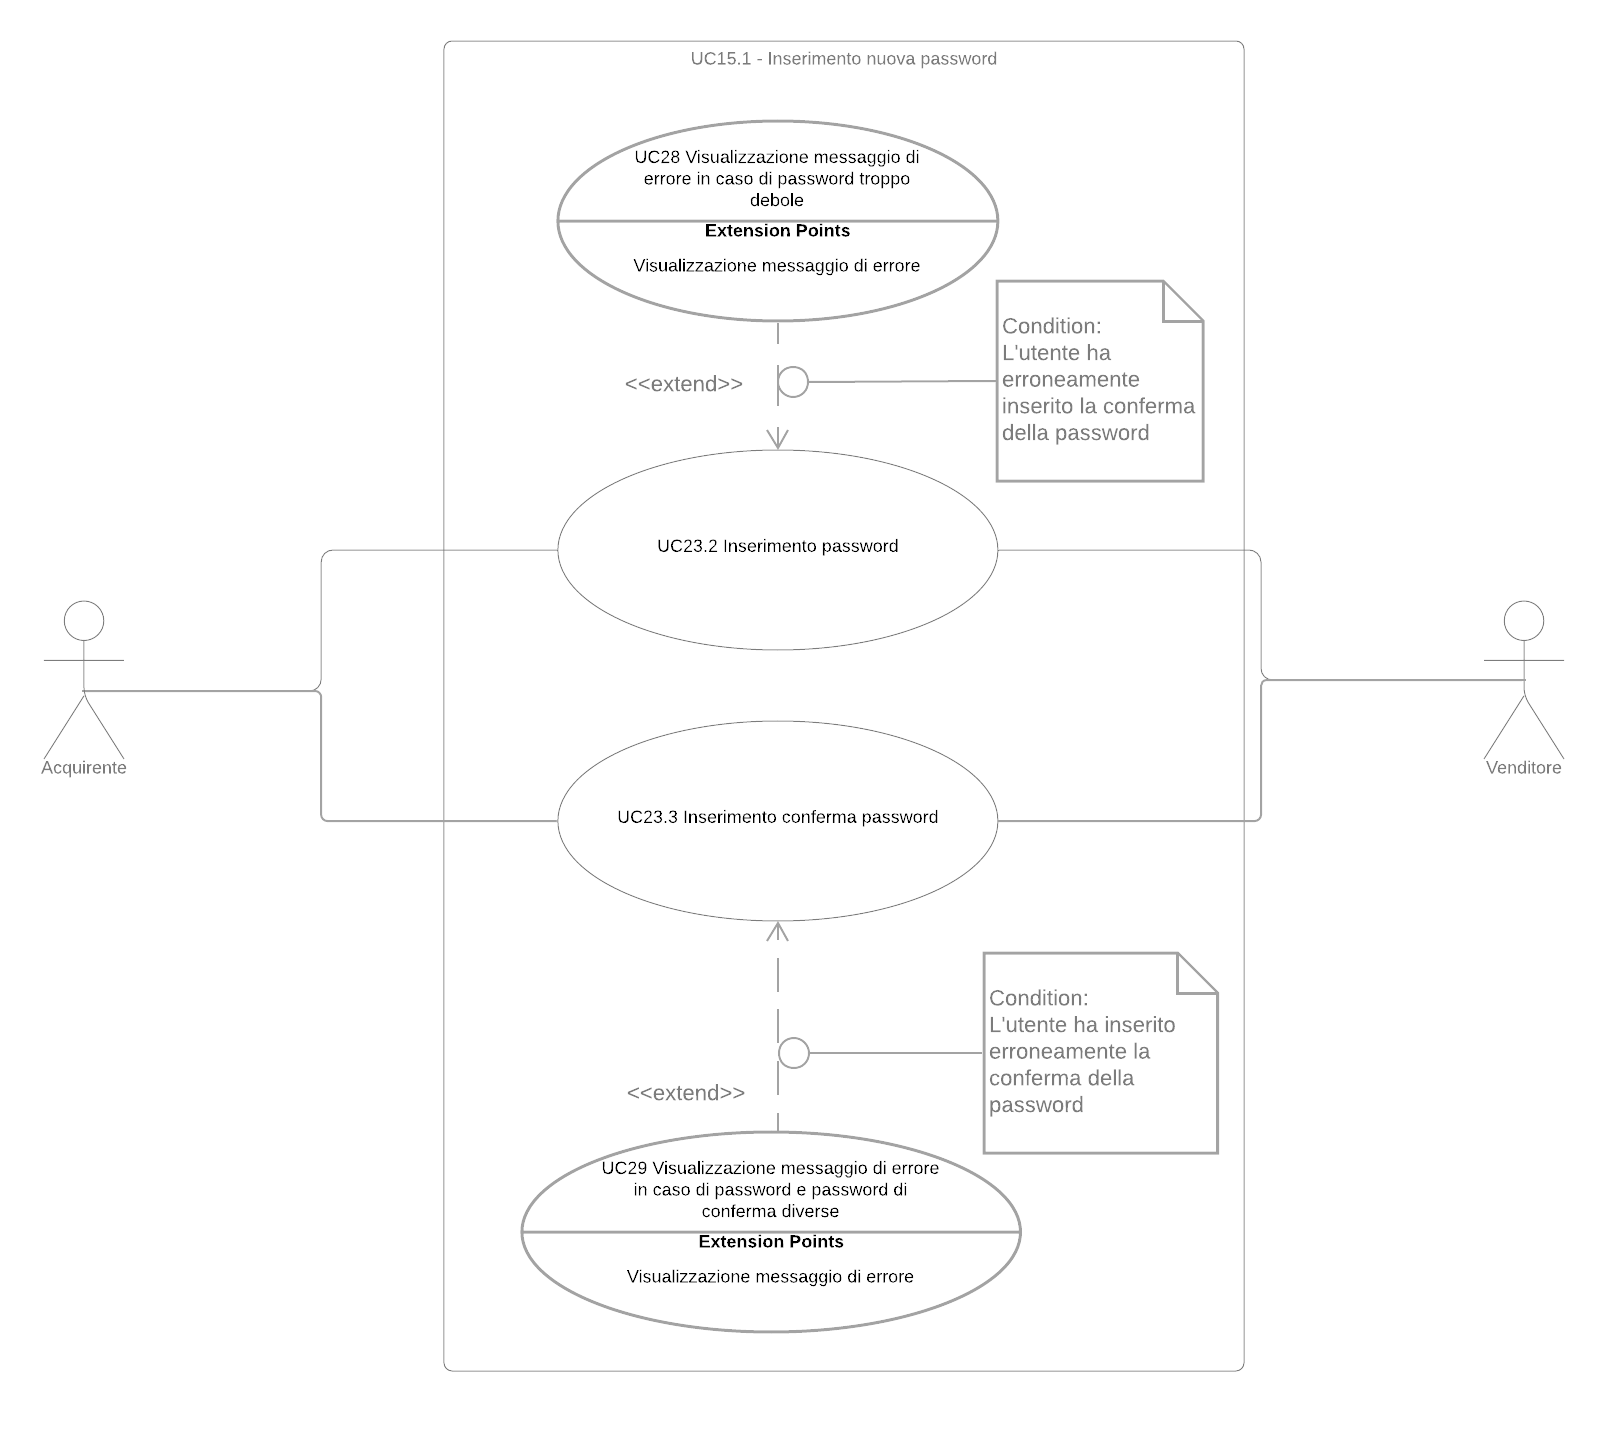
\includegraphics[width=\textwidth]{Immagini/DiagrammiUC/UC15.1InserimentoNuovaPassword}
    \caption{Diagramma di UC15.1: Inserimento nuova password} 
    \label{fig:VisualizzazioneProdottiNelCarrello}
\end{figure}

L'acquirente o il venditore vuole cambiare la password.
\begin{itemize}
    \item \textbf{Attori primari:} Acquirente; Venditore.
    \item \textbf{Precondizione:} L'attore ha premuto sul link per la modifica della password.
    \item \textbf{Postcondizione:} L'attore ha modificato la sua password.
    \item \textbf{Scenario Principale:} L'utente autenticato vuole cambiare la password e deve eseguire i seguenti passi:
    \begin{itemize}
        \item (UC23.2) - Inserimento password.
        \item (UC23.3) - Inserimento conferma password.
    \end{itemize}
    \item \textbf{Estensioni:}
    \begin{itemize}
        \item (UC28) - Visualizzazione messaggio di errore in caso di password troppo debole.
    \end{itemize}
\end{itemize}

\subsection{UC16 - Eliminazione account}
\label{UC16}
L'acquirente può eliminare il proprio account.
\begin{itemize}
    \item \textbf{Attori Primari:} Acquirente.
    \item \textbf{Precondizione:} L'acquirente si trova nella propria pagina personale (UC3.2.1) e ha selezionato l'azione di cancellazione del proprio account. 
    \item \textbf{Postcondizione:} L'account dell'acquirente non è più presente nella piattaforma
    \item \textbf{Scenario Principale:} L'acquirente vuole eliminare il proprio account e compie le seguenti operazioni:
    \begin{itemize}
        \item Preme sull'azione di cancellazione del proprio account.
        \item Viene visualizzato un messaggio di conferma dell'operazione.
        \item Se conferma viene eliminato l'account.
    \end{itemize}
    \item \textbf{Scenario Alternativo:} Se non conferma viene riportato alla propria pagina personale.
\end{itemize}

\subsection{UC17 - Visualizzazione ordini effettuati}
\label{UC17}
L'acquirente vuole vedere l'elenco degli ordini effettuati sulla piattaforma.
\begin{itemize}
    \item \textbf{Attori primari:} Acquirente.
    \item \textbf{Precondizione:} L'acquirente si trova nella pagina del suo profilo.
    \item \textbf{PostCondizione:} L'acquirente visualizza l'elenco degli ordini.
    \item \textbf{Scenario Principale:} L'utente, all'interno della pagina del profilo, vede l'elenco degli ordini effettuati.
        Per ogni ordine effettuato sono indicati i prodotti inclusi nell'ordine, la loro quantità e il prezzo totale pagato.
    \item \textbf{Scenario Alternativo:} L'utente non ha ancora effettuato ordini, viene visualizzato il messaggio "Nessun ordine effettuato" e sarà data la possibilità all'attore di andare alla home per iniziare gli acquisti.
\end{itemize}
